\documentclass{beamer}

\usepackage{amsmath, amssymb, graphicx, multicol, tikz, array}
\usepackage[absolute,overlay]{textpos}
\usepackage[export]{adjustbox}
\usepackage{pgfplots, pgf-pie}
\usetikzlibrary{positioning}
\usetikzlibrary{calc}
\pgfplotsset{compat=1.17}

% \usepackage{zxjatype}
% \usepackage[ipa]{zxjafont}
% \usepackage{mymacro}

\setbeamerfont*{itemize/enumerate body}{size=\large}
\setbeamerfont*{itemize/enumerate subbody}{parent=itemize/enumerate body}
\setbeamerfont*{itemize/enumerate subsubbody}{parent=itemize/enumerate body}

\usefonttheme{professionalfonts}
\setbeamertemplate{navigation symbols}{}

% --- page number ---
\setbeamertemplate{footline}{%
	\raisebox{10pt}{\makebox[\paperwidth]{\hfill\makebox[7em]{\normalsize\texttt{\insertframenumber/\inserttotalframenumber}}}}%
}

\DeclareMathOperator*{\argmin}{argmin}
\DeclareMathOperator*{\argmax}{argmax}
\DeclareMathOperator{\softmax}{softmax}
\DeclareMathOperator{\ReLU}{ReLU}

\title{Deep learning}
\subtitle{Probabilistic languange modeling with\\recurrent neural networks}
\author{Matthew Greenberg}
\date{May 2022}


\begin{document}

    \begin{frame}
    \maketitle
    \end{frame}
   
    \begin{frame}
        \frametitle{Probabilistic language models}

        \begin{itemize}
            \setlength\itemsep{1em}
            \item Represent text as a sequence of atomic \textbf{tokens},
            typically words or characters.

            \item Choose a \textbf{context size} $n>0$.
            
            \item Suppose that sequences $x_0,\ldots,x_{n-1},x_n$ of $n+1$
            consecutive tokens --- \textbf{$(n+1)$-grams} --- drawn from documents of a large text corpus
            are distributed according to
            \[
                P(x_n\mid x_0,\ldots,x_{n-1})
            \]

            \item Our modeling task is finding an approximation $\widehat{P}$ to $P$.
        \end{itemize}
    \end{frame}

    \begin{frame}
        \frametitle{The (n+1)-gram model}

        \begin{itemize}
            \setlength\itemsep{1em}
            \item Approximate the joint probability mass
            \[
                \widehat{P}(x_0,x_1,\ldots,x_n)
            \]
            by a relative frequency and setting
            \[
                \widehat{P}(x_n\mid x_0,\ldots,x_{n-1}) = \frac{\widehat{P}(x_0,\ldots,x_n)}
                {\widehat{P}(x_0,\ldots,x_{n-1})}.
            \]

            \item When $n=1$, this is called the \textbf{bigram model}.
            \item When $n=2$, this is called the \textbf{trigram model}.
        \end{itemize}
    \end{frame}

    \begin{frame}
        \frametitle{Text generation}

        \begin{itemize}
            \setlength\itemsep{1em}
            \item Having fit the $(n+1)$-gram model to a text corpus,
            we can generate new text by sampling from the model:
            \bigskip
            \begin{itemize}
            \setlength\itemsep{1em}
            \item Start with tokens $x_0,\ldots,x_{n-1}$.
            
            \item Draw $x_n$ from $\widehat{P}(x_n\mid x_0,\ldots,x_{n-1})$.
            \item Draw $x_{n+1}$ from $\widehat{P}(x_{n+1}\mid x_1,\ldots,x_n)$.
            \item \ldots
        \end{itemize}
    \end{itemize}
    \end{frame}

    \begin{frame}
        \frametitle{``Digestive'' language modeling}

        \bigskip

        \begin{itemize}
            \setlength\itemsep{1em}
            \item Suppose
        \[
            \widehat{P}(x_n\mid x_0,\ldots,x_{n-1}) = \widehat{P}(x_n\mid h_n),
        \]
        where $h_n$ is a ``digest'' of $x_0,\ldots,x_{n-1}$ that:

        \bigskip
        \begin{enumerate}
            \setlength\itemsep{1em}
            \item $h_n$ depends on $x_0,\ldots,x_{n-2}$ only through $h_{n-1}$, and
            \item the form of this dependence is independent of $n$:
            \[
                h_n = f(x_{n-1}, h_{n-1}).
            \]
        \end{enumerate}

        \item In practice, $f$ is a neural network.
    \end{itemize}

    \begin{center}
        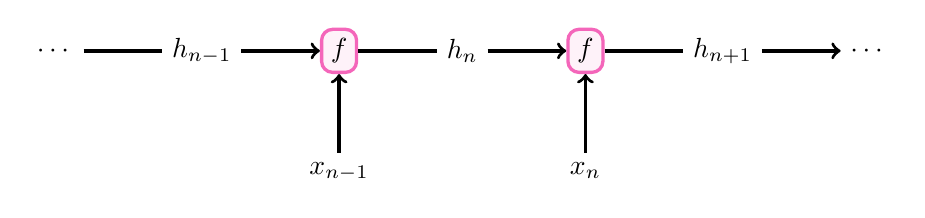
\begin{tikzpicture}[
            orangesquarednode/.style={rectangle, rounded corners, draw=orange!60, fill=orange!5, very thick},
            magentasquarednode/.style={rectangle, rounded corners, draw=magenta!60, fill=magenta!5, very thick},
            bluesquarednode/.style={rectangle, rounded corners, draw=blue!60, fill=blue!5, very thick},
            ]
            \node (P) {$\cdots$};
            \node[right=of P] (A) {$h_{n-1}$};
            \node[magentasquarednode, right=of A] (B) {$f$};
            \node[right=of B] (C) {$h_{n}$};
            \node[magentasquarednode, right=of C] (D) {$f$};
            \node[right=of D] (E) {$h_{n+1}$};
            \node[right=of E] (F) {$\cdots$};

            \node[below=of B] (XB) {$x_{n-1}$};
            \node[below=of D] (XD) {$x_{n}$};

            \draw[very thick] (P.east) -- (A.west);
            \draw[->, very thick] (A.east) -- (B.west);
            \draw[very thick] (B.east) -- (C.west);
            \draw[->, very thick] (C.east) -- (D.west);
            \draw[very thick] (D.east) -- (E.west);
            \draw[->, very thick] (E.east) -- (F.west);

            \draw[->, very thick] (XB.north) -- (B.south);
            \draw[->, very thick] (XD.north) -- (D.south);
        \end{tikzpicture}
    \end{center}
    \end{frame}

    \begin{frame}
        \frametitle{Training $f$}
        \bigskip
    
        \begin{itemize}
            \item We train $f$ to \textbf{predict the next token}, using an auxilliary classifier $g$, trained concurrently.
        \end{itemize}
    
        \begin{center}
            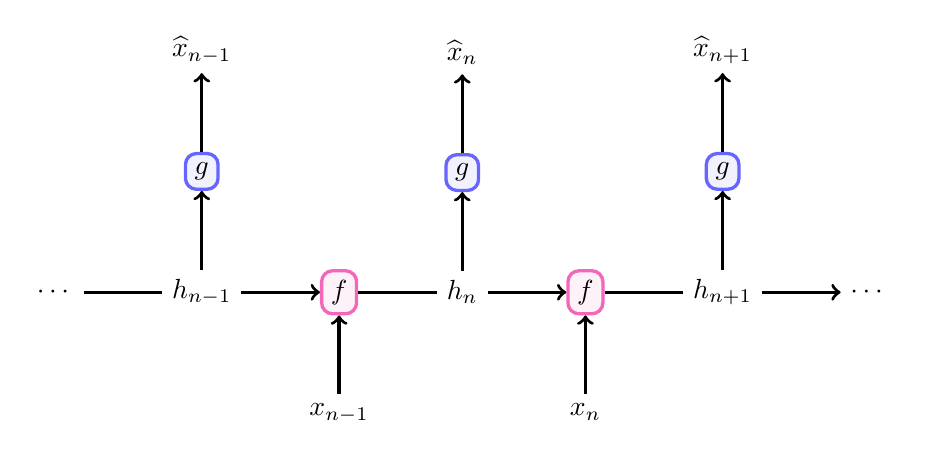
\begin{tikzpicture}[
                orangesquarednode/.style={rectangle, rounded corners, draw=orange!60, fill=orange!5, very thick},
                magentasquarednode/.style={rectangle, rounded corners, draw=magenta!60, fill=magenta!5, very thick},
                bluesquarednode/.style={rectangle, rounded corners, draw=blue!60, fill=blue!5, very thick},
                ]
                \node (P) {$\cdots$};
                \node[right=of P] (A) {$h_{n-1}$};
                \node[magentasquarednode, right=of A] (B) {$f$};
                \node[right=of B] (C) {$h_{n}$};
                \node[magentasquarednode, right=of C] (D) {$f$};
                \node[right=of D] (E) {$h_{n+1}$};
                \node[right=of E] (F) {$\cdots$};

                \node[below=of B] (XB) {$x_{n-1}$};
                \node[below=of D] (XD) {$x_{n}$};

                
                \node[bluesquarednode, above=of A] (GA) {$g$};
                \node[bluesquarednode, above=of C] (GC) {$g$};
                \node[bluesquarednode, above=of E] (GE) {$g$};
                
                \node[above=of GA] (XA) {$\widehat{x}_{n-1}$};
                \node[above=of GC] (XC) {$\widehat{x}_{n}$};
                \node[above=of GE] (XE) {$\widehat{x}_{n+1}$};

                \draw[very thick] (P.east) -- (A.west);
                \draw[->, very thick] (A.east) -- (B.west);
                \draw[very thick] (B.east) -- (C.west);
                \draw[->, very thick] (C.east) -- (D.west);
                \draw[very thick] (D.east) -- (E.west);
                \draw[->, very thick] (E.east) -- (F.west);

                \draw[->, very thick] (XB.north) -- (B.south);
                \draw[->, very thick] (XD.north) -- (D.south);

                \draw[->, very thick] (A.north) -- (GA.south);
                \draw[->, very thick] (C.north) -- (GC.south);
                \draw[->, very thick] (E.north) -- (GE.south);
                \draw[->, very thick] (GA.north) -- (XA.south);
                \draw[->, very thick] (GC.north) -- (XC.south);
                \draw[->, very thick] (GE.north) -- (XE.south);
            \end{tikzpicture}
        \end{center}
    \end{frame}

    \begin{frame}
        \begin{itemize}
            \setlength\itemsep{1em}
            \item We train RNNs on \textbf{batches} of \textbf{token sequences}.
            \item Training one sequence with inputs $x_0,\ldots,x_{s-1}$
            and targets $x_1,\ldots,x_s$:
        \end{itemize}
    
        \bigskip
        \begin{center}
            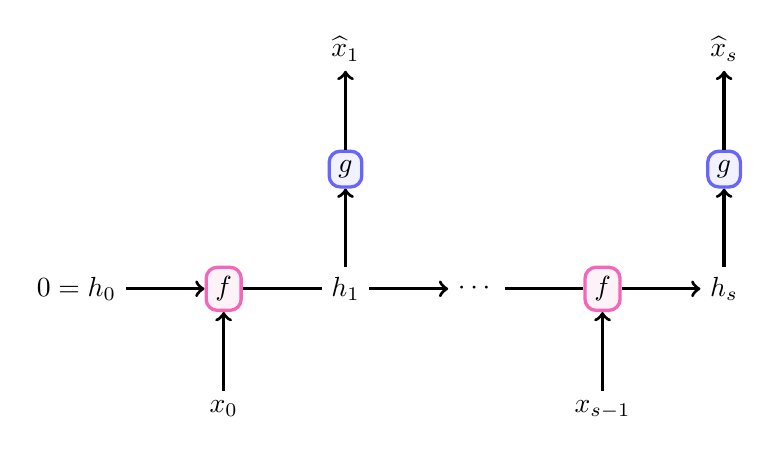
\begin{tikzpicture}[
                orangesquarednode/.style={rectangle, rounded corners, draw=orange!60, fill=orange!5, very thick},
                magentasquarednode/.style={rectangle, rounded corners, draw=magenta!60, fill=magenta!5, very thick},
                bluesquarednode/.style={rectangle, rounded corners, draw=blue!60, fill=blue!5, very thick},
                ]
                \node(A) {$0=h_0$};
                \node[magentasquarednode, right=of A] (B) {$f$};
                \node[right=of B] (C) {$h_{1}$};
                \node[right=of C] (D) {$\cdots$};
                \node[magentasquarednode, right=of D] (E) {$f$};
                \node[right=of E] (F) {$h_s$};

                \node[below=of B] (XB) {$x_{0}$};
                \node[below=of E] (XE) {$x_{s-1}$};

                
                \node[bluesquarednode, above=of C] (GC) {$g$};
                \node[bluesquarednode, above=of F] (GF) {$g$};
                
                \node[above=of GC] (XC) {$\widehat{x}_{1}$};
                \node[above=of GF] (XF) {$\widehat{x}_{s}$};

                \draw[->, very thick] (A.east) -- (B.west);
                \draw[very thick] (B.east) -- (C.west);
                \draw[->, very thick] (C.east) -- (D.west);
                \draw[very thick] (D.east) -- (E.west);
                \draw[->, very thick] (E.east) -- (F.west);

                \draw[->, very thick] (XB.north) -- (B.south);
                \draw[->, very thick] (XE.north) -- (E.south);

                \draw[->, very thick] (C.north) -- (GC.south);
                \draw[->, very thick] (F.north) -- (GF.south);
                \draw[->, very thick] (GC.north) -- (XC.south);
                \draw[->, very thick] (GF.north) -- (XF.south);
            \end{tikzpicture}
        \end{center}
    \end{frame}

    \begin{frame}
        \frametitle{Text generation}
    
        \begin{itemize}
            \setlength\itemsep{1em}
        \item We have:
        \begin{align*}
            h_n &= f(x_{n-1}, h_{n-1}),\\[0.5em]
            \widehat{P}(x_n\mid h_n) &= g(h_n)
        \end{align*}

        \item Having trained $f$ and $g$, we can generate text, autoregressively, as before.
    \end{itemize}
    
    \end{frame}

\end{document}
